\chapter{The FAT16 File System and Its Emulation} \label{sec:fat16}

A \gls{FS} is used by GEX to provide a comfortable access to the configuration files. By emulating a Mass Storage \gls{USB} device, the module appears as a thumb drive on the host \gls{PC}, and the user can edit its configuration using their preferred text editor. The FAT16 file system was selected for its simplicity and a good cross-platform support.

Three variants of the \gls{FAT} file system exist: FAT12, FAT16, and FAT32. FAT12 was used on floppy disks and it is similar to FAT16, except for additional size constraints and a \gls{FAT} entry packing scheme. FAT16 and FAT32 are FAT12's later developments from the time when hard disks became more common and the old addressing scheme couldn't support their larger capacity.

This chapter will explain the structure of FAT16 and the challenges faced when trying to emulate it without a physical data storage.

\section{The General Structure of the FAT File System}

The storage medium is organized into \textit{sectors} (or \textit{blocks}), usually 512 bytes long. Those are the smallest addressing unit in the disk structure. The disk starts with a \textit{boot sector}, also called a \gls{MBR}). That is followed by optional reserved sectors, one or two copies of the file allocation table, and the root directory. All disk areas are aligned to a sector boundary:

\begin{table}[h]
	\centering
	\begin{tabular}{ll}
		\toprule
		\textbf{Disk area} & \textbf{Size / Notes} \\
		\midrule
		Boot sector & 1 sector \\
		Reserved sectors & optional \\
		FAT 1 & 1 or more sectors, depends on disk size \\
		FAT 2 & optional, a back-up copy of FAT 1 \\
		Root directory & 1 or more sectors \\
		Data area & Organized in \textit{clusters} \\
		\bottomrule
	\end{tabular}
	\caption{\label{tab:fat16-disk-areas}Areas of a FAT-formatted disk}
\end{table}

\subsection{Boot Sector}

This is a 1-sector structure which holds the \gls{OS} bootstrap code for bootable disks. The first 3 bytes are a jump instruction to the actual bootstrap code located later in the sector. What matters to us when implementing the file system is that the boot sector also contains data fields describing how the disk is organized, what file system is used, who formatted it, etc. The size of the \gls{FAT} and the root directory is defined here. The exact structure of the boot sector can be found in XXX\todo{add ref link} or in the attached GEX source code.

\subsection{File Allocation Table}

The data area of the disk is organized in clusters, logical allocation units composed of groups of sectors. The use of a larger allocation unit allows the system to use shorter addresses and thus support a larger disk capacity.

The \gls{FAT} acts as a look-up table combined with linked lists. In FAT16, it is organized in 16-bit fields, each corresponding to one cluster. The first two entries in the allocation table are reserved and hold special values set by the disk formatter and the host \gls{OS}: a "media descriptor" 0xFFF8 and a "clean/dirty flag" 0xFFFF/0x3FFF.

Files can span multiple clusters; each \gls{FAT} entry either holds the address of the following file cluster, or a value with a special meaning:

\begin{itemize}
	\item 0x0000 - free cluster
	\item 0xFFFF - last cluster of the file (still including file data!)
	\item 0xFFF7 - bad cluster
\end{itemize}

The bad cluster mark, 0xFFF7, is used for clusters which are known to corrupt data due to a flaw in the storage medium, such us a bad memory cell.

\subsection{Root Directory}

The root directory has the same structure as any other directories, which reside in clusters the same way like ordinary files. The difference is that the root directory is allocated when the disk is formatted and it has a fixed and known position and size. Sub-directories are stored on the disk in a similar way to regular files, therefore they can span multiple sectors and their file count can be much larger than that of the root directory.

\begin{table}
	\centering
	\begin{tabular}{lll}
		\toprule
		\textbf{Offset} & \textbf{Size (bytes)}  & \textbf{Description}\\
		\midrule
		0 & 8 & File name (padded with spaces) \\
		8 & 3 & File extension \\
		11 & 1 & File attributes \\
		12 & 10 & Reserved \\
		22 & 2 & Creation time \\
		24 & 2 & Creation date \\
		26 & 2 & Address of the first cluster \\
		28 & 4 & File size (bytes) \\
		\bottomrule
	\end{tabular}
	\caption{\label{tab:fat16-dir-entry}Structure of a FAT16 directory entry}
\end{table}

A directory is organized in 32-byte entries representing individual files. Table \ref{tab:fat16-dir-entry} shows the structure of one such entry.

The name and extension fields form together the well-known 8.3 filename format. Longer file names are encoded using a \gls{LFN} scheme as special hidden entries stored in the directory table alongside the regular 8.3 entries, ensuring backward compatibility.

The first byte of the file name has a special meaning:

\begin{itemize}
	\item 0x00 - indicates that there are no more files when searching the directory
	\item 0xE5 - marks a free slot; this is used when a file is deleted
	\item 0x05 - indicates that the first byte should actually be 0xE5, which was used in a Japanese character set.
	\item Any other value, except 0x20 (space) and characters forbidden in a DOS file name, starts a valid file entry. Generally, only space, A-Z, 0-9, \verb|-| and \verb|_| should be used in file names for maximum compatibility.
\end{itemize}

The attributes field contains flags such as \textit{directory}, \textit{volume label}, \textit{read-only} and \textit{hidden}. Volume label is a special entry in the root directory, which defines the disk's label shown on the host \gls{PC}. A file with the directory bit set is actually a pointer to a subdirectory, meaning that when we open the linked cluster, we'll find a new directory table.

Figure \ref{fig:fat-example} shows a possible organization of the GEX file system with two INI files, one spanning two clusters, the other being entirely inside one. The clusters need not be used completely; an exact file size is stored in the directory entries.

\begin{figure}[h]
	\centering
	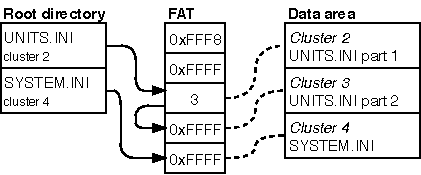
\includegraphics[scale=1.3] {img/fat-links.pdf}
	\caption{\label{fig:fat-example}An example of the GEX virtual file system}
\end{figure}


\section{FAT16 Emulation}

The FAT16 file system is relatively straightforward and easy to implement. This is the reason why an emulation driver for it was developed as part of the open-source ARM mbed DAPLink project. \todo{reference} It is used there for a drag-and-drop flashing of firmware images to the target microcontroller, taking advantage of it working well across different host platforms. ARM mbed uses a browser-based \gls{IDE} and cloud build servers, thus the end user does not need to install or set up any software or drivers to program a compatible development kit. The GEX firmware adapts several parts of this code, optimizes its \gls{RAM} usage and further expands its functionality to support our specific use case.

It is not practical or even possible to keep the entire file system in memory, especially with a microcontroller like the STM32F072, which has only 16\,kB of \gls{RAM} in total. This means that we have to generate and parse disk sectors and clusters on-demand, when the host reads or writes them. The STM32 \gls{USB} Device library helpfully implements the \gls{MSC} and provides \gls{API} endpoints to which we connect our file system emulator. Specifically, those are requests to read and write a sector, and to read disk status and parameters, such as its size.

As shown in table \ref{tab:fat16-disk-areas}, the disk consists of several areas. The boot sector is immutable and can be stored in Flash. The handling of the other areas (\gls{FAT}, data area) depends on whether we're dealing with a read or write access:

\subsection{Handling a Read Access}

The user can only read files that already exist on the disk, in our case, \verb|UNITS.INI| and \verb|SYSTEM.INI|. Those files are generated from the binary settings storage, and conversely, parsed, line-by-line, without ever existing in their full form. This fact makes our task more challenging, as the files can't be easily measured and there's no obvious way to read a sector from the middle of a longer file. We solve this by implementing two additional functions in the INI file writer: a \textit{read window} and a \textit{dummy read mode}.

A read window is a byte range which we wish to generate. The INI writer discards bytes before the start of the read window, writes those inside the window to our data buffer, and stops when its end is reached. This lets us extract a sector from anywhere in a file. The second function, dummy read, is tied to the window function: we set the start index so high that it's never reached (e.g. 0xFFFFFFFF), and have the writer count discarded characters. When the dummy file generation ends, this character counter holds its size.

Now, just one problem remains: how to tell which sectors contain which part of our files? This is straightforward when we realize that the files change only when the user modifies the settings. After each such change, an algorithm is run which allocates clusters to the files and preserves this information in a holding structure. A subsequent read access simply requires a look into this structure and the corresponding chunk of a file may be served using the read window function. The \gls{FAT} can be dynamically generated from this information as well.

\subsection{Handling a Write Access}

A file write access is more challenging to emulate than a read access, as the host OS tends to be somewhat unpredictable. In GEX's case we're interested only in the action of overwriting an already existing file, but it's interesting to also analyze other actions the host may perform.

It must be noted that due to the nonexistence of a physical storage medium, it's not possible to read back a file the host has written. The \gls{OS} may show the written file on the disk, but when the user tried to read it, it either fails, or shows a cached copy. In the DAPLink emulator this is worked around by temporarily reporting that the storage medium has been removed, forcing the host to re-load its contents. In GEX, the loaded INI file will be a newly generated copy, embedding possible error messages as comments.

\subsubsection{File Deletion}

A file is deleted by:

\begin{enumerate}
	\item Marking all sectors used by it as free in the \gls{FAT}
	\item Replacing the first character of its name in the directory table by 0xE5 to indicate the slot is free
\end{enumerate}

From the perspective of emulation, we can ignore the \gls{FAT} access and only detect writes to the directory sectors. This is slightly more complicated when one considers that all disk access is performed in sectors: the emulator must compare the written data with the original bytes to detect what change has been performed. Alternatively, we could parse the written sector as a directory table and compare it with our knowledge of its original contents.

\subsection{File Name Change}

A file is renamed by modifying its directory entry. This can be be detected in a similar way to a file deletion. In the simple case of a short, 8.3 file name, this is a in-place modification of the file entry. Long file names, using the \gls{LFN} extension, are a complication, as the number of dummy entries might change when the file name is shortened or made longer, and subsequently the following entries in the table may shift or be entirely re-arranged.

\subsection{File Creation}

A new file is created in three steps:

\begin{enumerate}
	\item Finding free clusters and chaining them by writing the following cluster addresses (or 0xFFFF for the last cluster) into the \gls{FAT}
	\item Finding and overwriting a free entry in the directory table
	\item Writing the file content
\end{enumerate}

It can be expected the host \gls{OS} first finds the free sectors and a free file entry before performing any write operations, to prevent a potential disk corruption.

To properly handle such a file by the emulator, we could, in theory, find its name from the directory table, which has been updated, and then collect the data written to the corresponding clusters. In practice, confirmed by experiments with a real Linux host, those three steps may happen in any order, and often the content is written before the directory table is updated.

The uncertain order of the written disk areas poses a problem when the file name has any significance, as we can't store the received file data while waiting for the name to be written. The DAPLink mbed flashing firmware solves this by analyzing the content of the first written sector of the file, which may contain the binary \gls{NVIC} table, or a character pattern typical for Intel hex files.

\subsection{File Content Change}

A change to a file's content is performed in a similar way to the creation of a new file, except instead of creating a new entry in the directory table, an existing one is updated with the new file size. The name of the file may be, again, unknown until the content is written, but we could detect the file by comparing the starting sector with those of all files known to the virtual file system.

In the case of GEX, the detection of a file name is not important; we expect only INI files to be written, and the particular file may be detected by its first section marker, such as \verb|[UNITS]| or \verb|[SYSTEM]|. Should a non-INI file be written by accident, the INI parser will likely detect a syntax error and discard it.

It should be noted that a file could be updated only partially, skipping the clusters which remain unchanged, and there's also no guarantee regarding the order in which the file's sectors are written. This is hard to detect and handle and the current firmware is not able to interpret it correctly, thus such a write operation will fail. Fortunately, this host behavior has not been conclusively observed in practice, but a write operation rarely fails for still unknown reasons and this could be a possible cause.







































